\section{Experiments} \label{sec:experiments}

Toward the goal of evaluation on a current challenge dataset, we spent time to setup the baselines, before proceeding with learning approaches.
Here we report the baseline, and describe the next step in that direction.

To explore appropriate learning methods for the problem, we developed a toy problem that represents the salient details of the full image detection tasks.
Here we report our initial experiments, using a model-free batch reinforcement learning method.

\subsection{PASCAL Baseline}
Among published detection frameworks, the Cascaded DPM detector~\cite{Felzenszwalb2010b} has probably the highest performance to speed ratio.
To use it as a baseline, we had to first evaluate it in the AP vs. Time regime as described in~\autoref{sec:evaluation}.

Toward this end, we write out detections as each stage of the cascade is passed, at each location, for each class.
This of course results in far too many detection hypotheses.
To reduce them to a reasonable set that would lead to the best performance according to the PASCAL criterion, we employ the standard technique of Non-Maximum Suppression (NMS), where two overlapping detections are reduced to just one: the detection with the higher score.
Specifically: at discrete time intervals, we pool all surviving detection hypotheses from previous intervals, add in new ones from the current interval, and run NMS.
The resulting set of detections is evaluated and measured by the Average Precision.

\begin{figure}[h!]
  \centering
\subfloat[Example of performance on a single image.]{
\label{fig:apvst_example}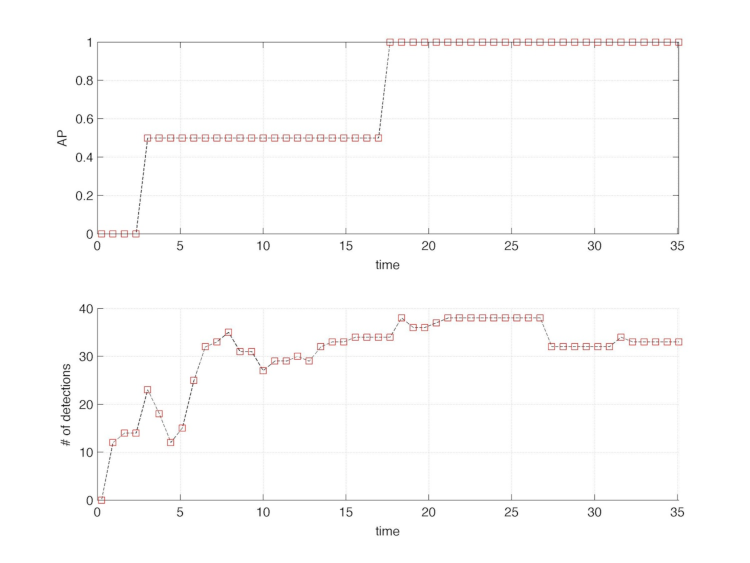
\includegraphics[width=0.75\textwidth]{../figures/example_apvst_plot.pdf}}
\\
\subfloat[Average performance across the dataset. Gray area is bounded by one standard deviation away from the mean.]{\label{fig:apvst_baseline}  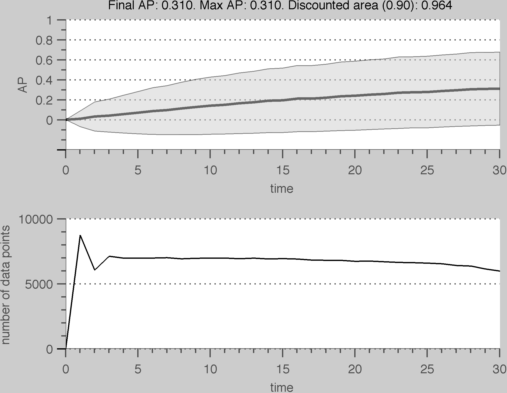
\includegraphics[width=0.75\textwidth]{../figures/apvst_baseline.png}}
  \caption{Plot of baseline performance of the Cascaded DPM Detector~\cite{Felzenszwalb2010b}, in the AP vs. Time evaluation regime.}
  \label{fig:apvst_baselines}
\end{figure}

\begin{figure}[h!]
  \centering
    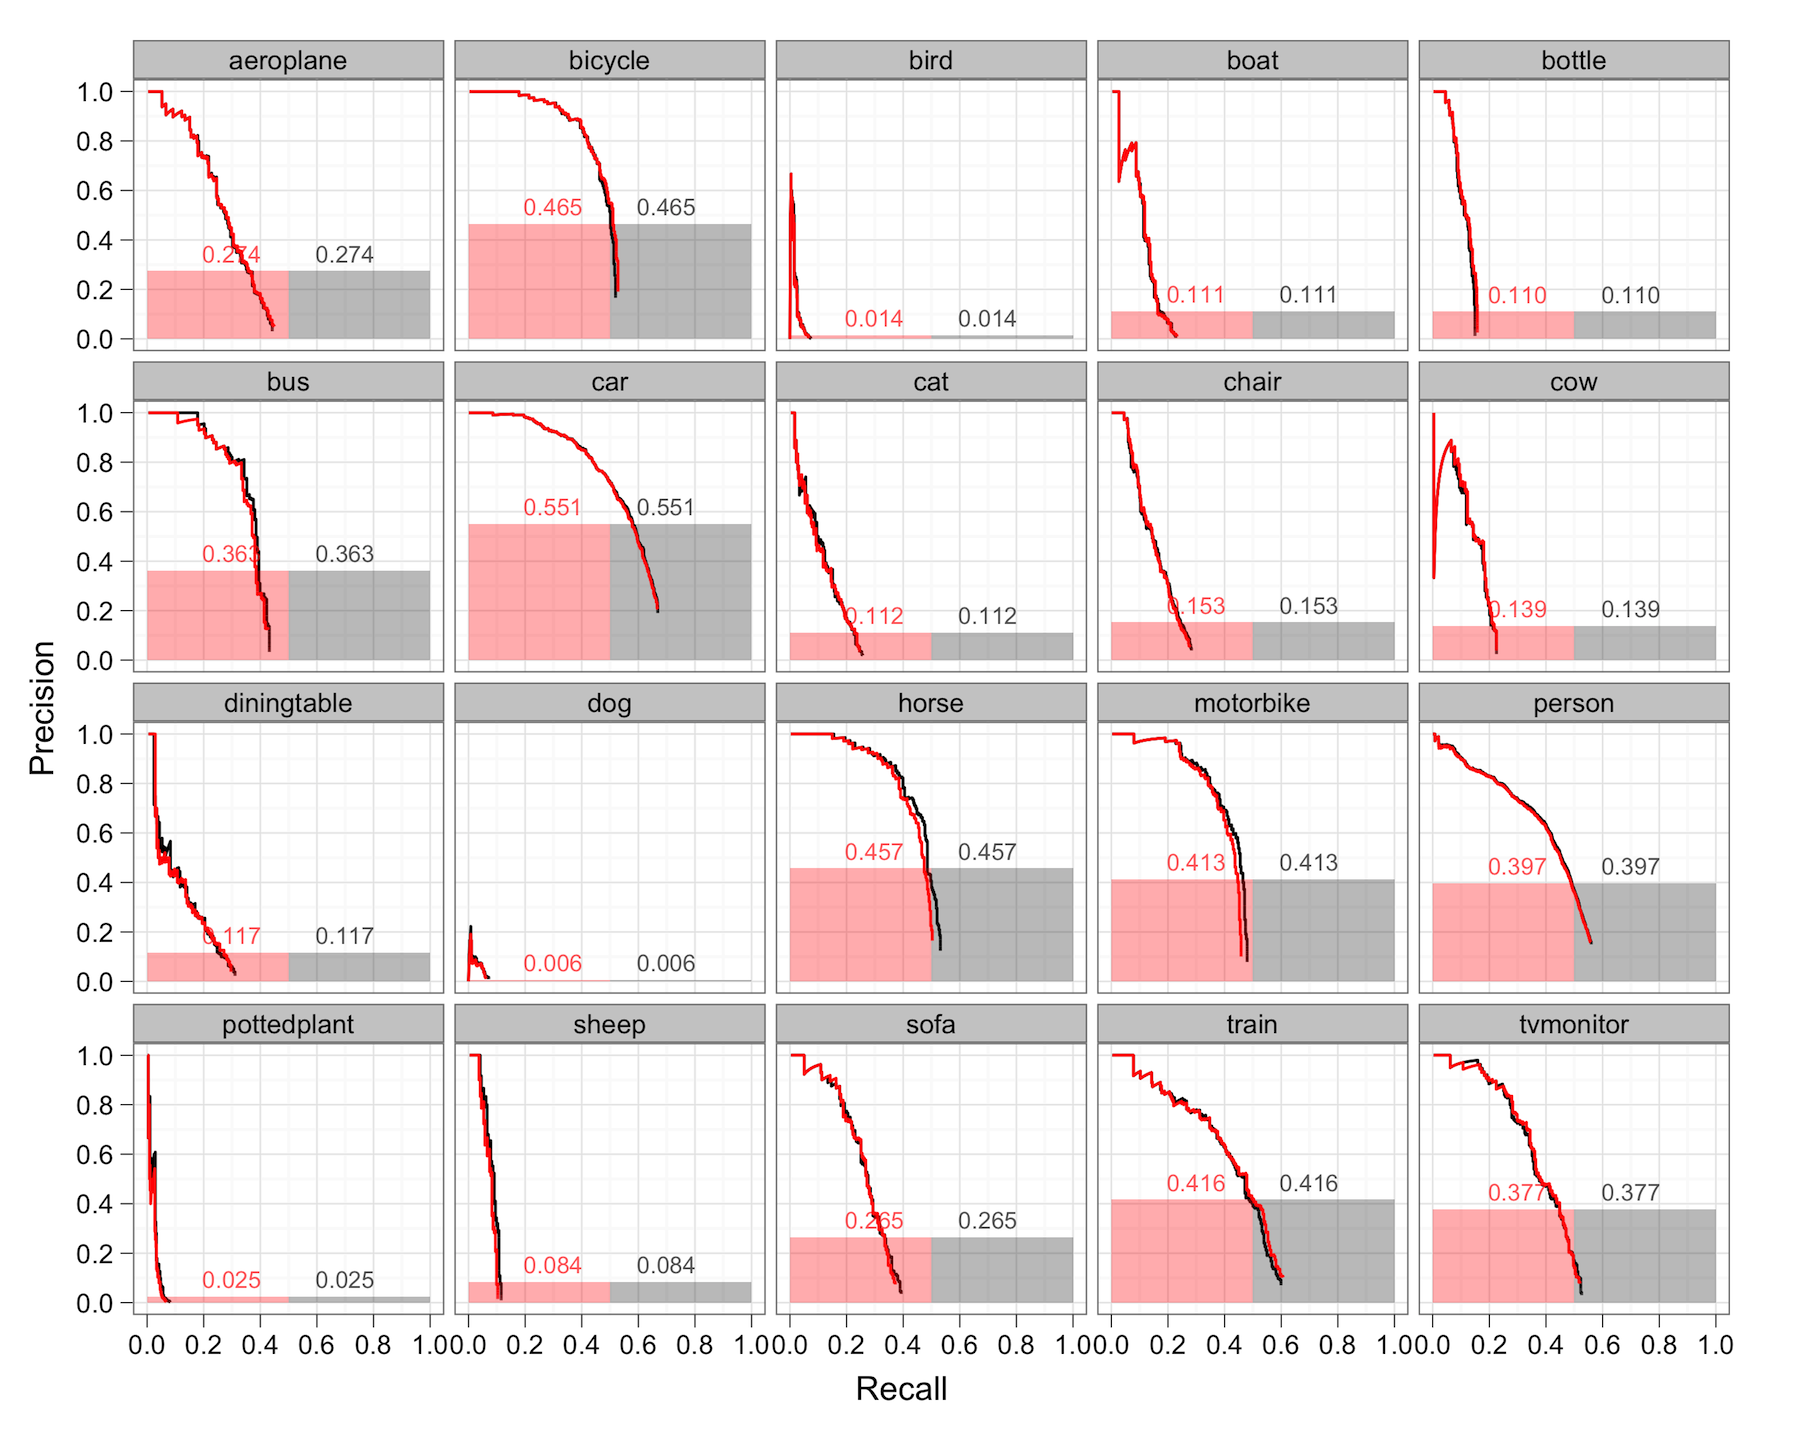
\includegraphics[width=0.9\textwidth]{../figures/pr_grid_comparison.png}
  \caption{Our method of computing Anytime detections results in final detections that perform as well as the final output of the cascade.}
  \label{fig:pr_grid_comparison}
\end{figure}

Figure~\ref{fig:apvst_baselines} shows a typical AP vs. T plot for a single image, and the same data averaged across all images in the test dataset.
Note the slope of rise to the final AP score; our goal is to make this steep leading up to some deadline, and either plateau (if final AP is reached) or increase to final AP after that.
We can formulate the desired performance as a scalar measure: the discounted AP starting at deadline.
We note that to construct these evaluations, we had to pick an ordering over classes.
To remove the effect of a particular ordering being better suited to the dataset, we randomized the ordering for each image.
Figure~\ref{fig:pr_grid_comparison} shows that this method of evaluation results in final detections that achieve the same level of performance as if the cascade had run un-interrupted to completion.

The baseline represents the output of a particular policy that samples locations and classes in a fixed order.
We can find the optimal order for the validation dataset by exhaustive search; that would produce an optimal baseline for the policy class.
This is current work, along with a simple novel policy of sampling in order from a saliency map computed on the image, as described in~\autoref{sec:example_policies}.

\subsection{Toy problem}
To experiment with different reinforcement learning problem formulations, we created a toy problem.
In it, we consider an image with $N$ locations, with some number of locations containing objects of some class $\{1:K\}$.
For initial experiments, we assume that we have perfect classifiers, so if a detect action is run, we become fully certain about the presence of the examined class at the examined location.
This is a simplifying assumption about the detectors, that moves the problem away from the domain of POMDPs.
Still, as described in~\autoref{sec:misc}, an Augmented MDP representation of the original problem is roughly the same as this formulation, except with an unknown, stochastic reward function.

To be able to generalize to large state and action spaces, and to the Augmented MDP formulation, we use the model-free Least Squares Policy Iteration approach~\cite{Lagoudakis2003}.
The approach consists of two parts.

First, linear function approximation is used for the $Q$ function, such that:
\begin{equation}
  Q^\Pi(s,a) \approx \hat{Q}^\Pi(s,a) = \sum_{i=1}^k \phi_i(s,a)w_i = \phi(s,a)^Tw
\end{equation}

LSPI learns the weights $w$, which fully determine the policy $\pi$ using batch temporal difference learning.
First, the agent interacts with the environment following some (at first random) policy to generate samples $<s,a,r,s'>$, with the obvious meanings.
The tuples are used to update a $k \times k$ matrix $A$ and $k \times 1$ vector $b$:
\begin{align}
A &\leftarrow A + \phi(s,a)(\phi(s,a)^T - \gamma \phi(s',\pi(s'))^T) \\
b &\leftarrow b + \phi(s,a)r
\end{align}

The weights vector $w$ can be extracted by solving $A^{-1}b$.
The learning procedure (1) generates $S$ samples by following the current policy, beginning with random; (2) updates the current policy by first setting $A,b$ to $0$, updating them with the samples as above, an deriving the new policy; (3) repeating step (2) until the error between two sequential policy vectors is $< \delta$; (4) generating new samples by following an $\epsilon$-greedy policy.
This procedure was followed for an active learning problem~\cite{Kwok2004}.

LSPI is an off-policy algorithm that is able to use the same set of samples to improve the policy at each iteration of step (2).
It converges faster and with less samples than TD($\lambda$) or SARSA($\lambda$), due to its least squares formulation.

As mentioned in~\autoref{sec:actions}, we face two distinct ways to define the action space.
For initial experiments, we chose the fully general action space, such that $|A| = NK$, meaning that any detector can be run at any location.

The $k$ features are designed manually.
For each action, we learn a separate Q-function (given $a$, $\phi(s,a)$ is only non-zero at locations corresponding to $a$).
The feature vector is simple:
\begin{equation}
  \phi(s,a) = <E_i, 1>
\end{equation}
$E_i$ is a binary feature that is $1$ if the (location,class) pair given by $a$ has been examined, according to our internal state $s$, and $-1$ otherwise.
$1$ is a constant allowing the policy to select actions.
$w$ therefore has $2NK$ parameters.

\begin{figure}[h!]
  \centering
    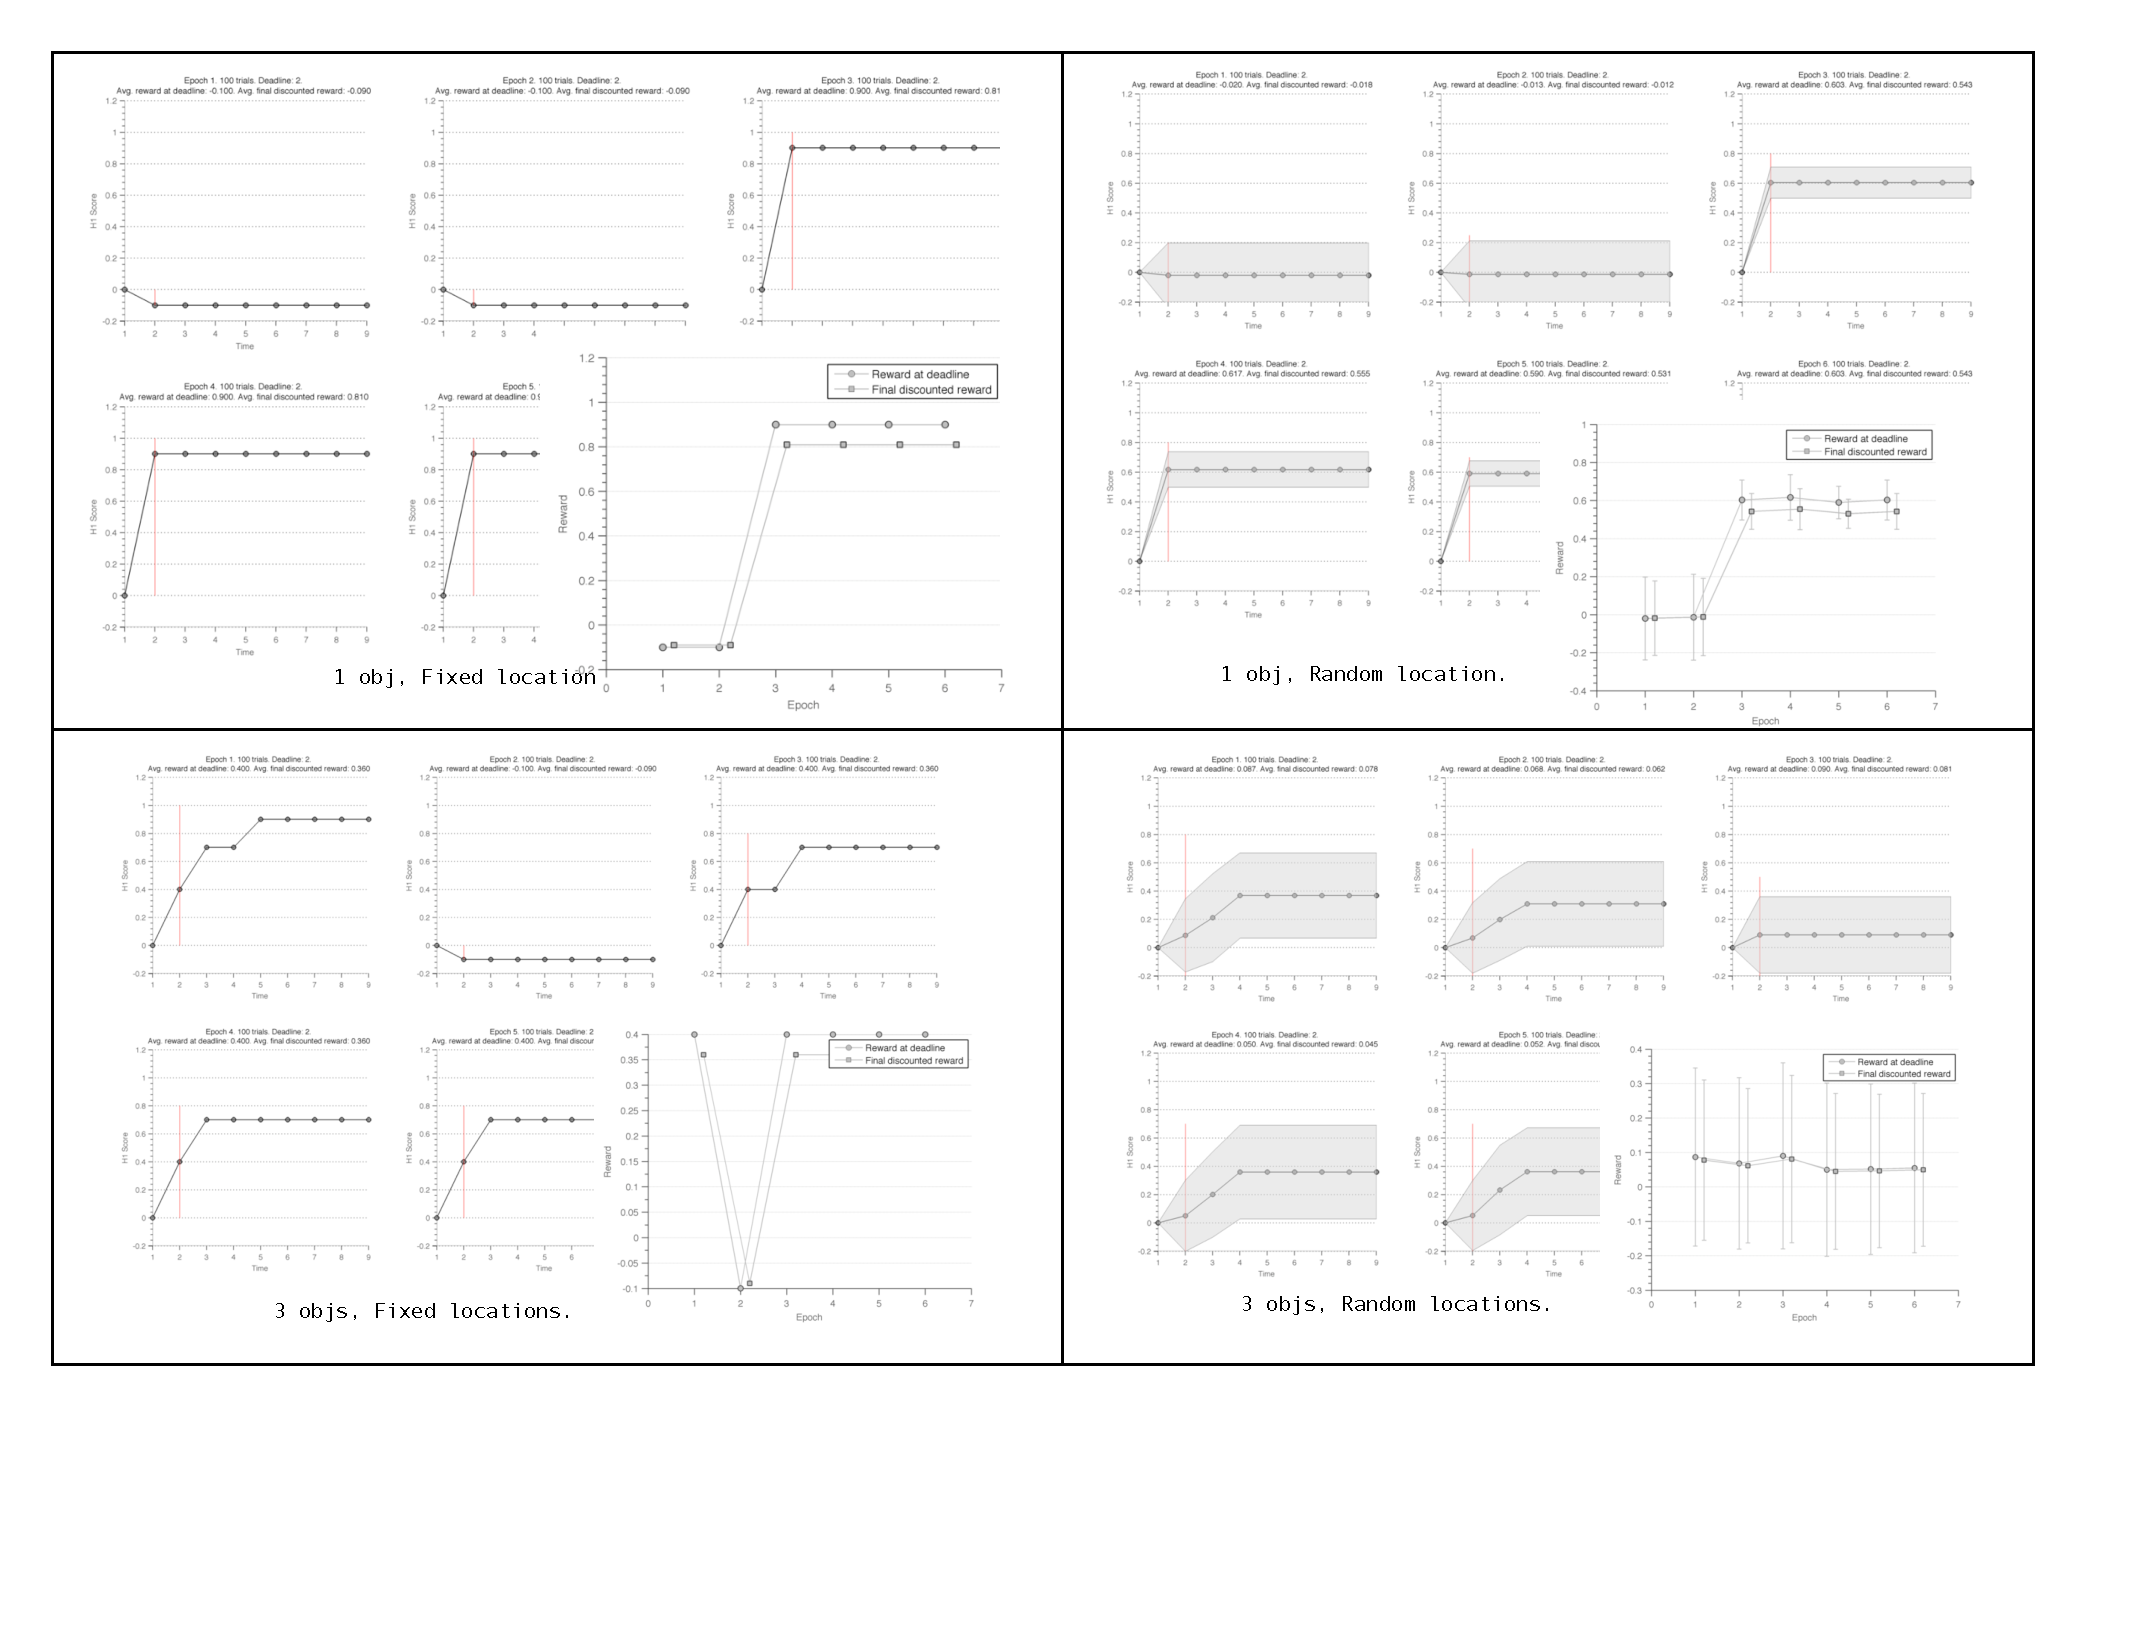
\includegraphics[width=1\textwidth]{../figures/rl.pdf}
  \caption{Some initial experiments using LSPI to solve the toy problem described here. The approach easily learns to find one object at a fixed location, and performs well with random single-object placement. It does not recover multiple objects at fixed locations successfully, and sometimes struggles when they are randomly placed. These are initial experiments, in ongoing work.}
  \label{fig:rl}
\end{figure}
In Figure~\ref{fig:rl}, we show the results of our initial experiments with learning a policy. We are able to learn policies for deterministically or probabilistically-placed object classes.
The learning appears to be heavily influenced by having enough samples from a random policy; we keep $\epsilon$ high such that even stable policies generate enough random samples.
In general, a lot of parameter tuning is needed for successful learning, and this is something we are still actively exploring.
We have not yet tried to learn policies corresponding to more complicated object placement rules.

We attribute some of the difficulty of learning a successful policy partly to the highly complex action space.
In current experiments, we are considering actions of a more restricted class, such as ``pick a random unexamined (location,class) pair.''